% ------------------------------------------------------------------------
% file `main-bookexercise-6-solution-body.tex'
%
%     solution of type `bookexercise' with id `6'
%
% generated by the `exerciseanswer' environment of the
%   `xsim' package v0.21 (2022/02/12)
% from source `main' on 2026/10/23 on line 729
% ------------------------------------------------------------------------
1. 选B。顶点A与顶点E存在相互连通的路径: A -> D -> E 以及 E -> D -> A，选项B错误。\\

2. 选D。A项，存在两顶点A、E，A到E无路径，所以$G_1$不是强连通的；对于$G_2$，F到G无路径，因此$G_2$不是强连通的；$G_3$任意两顶点之间都有路径，是强连通的。B项，
图$G$存在以下强连通分量：
\begin{center}
    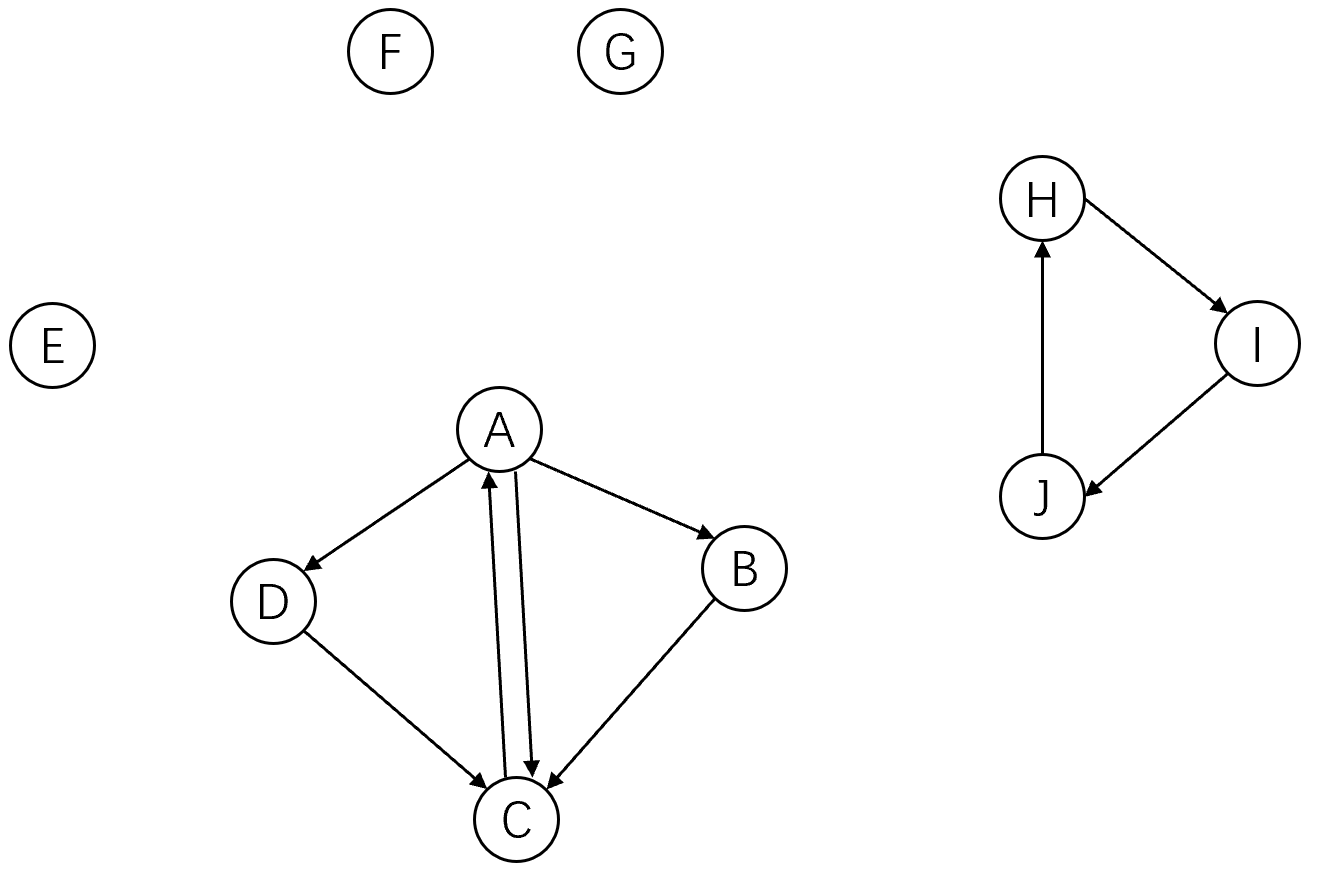
\includegraphics[width=0.58\textwidth]{assets/pics_and_ppts/ch5/习题02，图的基本概念答案图.png}
\end{center}
显然数量大于3。C项，顶点A出度为3，入度为1，C正确。D项，顶点F出度为0，入度为1，D错误。\\

3. 选A。下图所示的图是一个无向连通图，但不具有\(\mathrm{II}\)与\(\mathrm{III}\)的特性。只有\(\mathrm{I}\)正确。
\begin{center}
    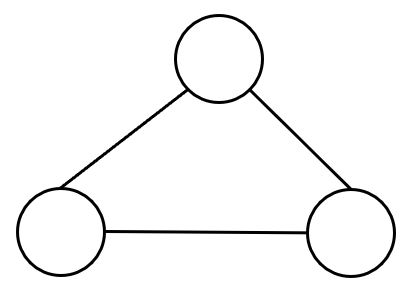
\includegraphics[width=0.19\textwidth]{assets/pics_and_ppts/ch5/习题03，09408无向连通图特性答案图.png}
\end{center}

\vspace{\baselineskip}

4. 要使得边数达到最大，一定是任意两个顶点之间都有一条边。因此最大边数是从N个顶点选出2个的组合数：
\[
    C_N^2 = \frac{N(N-1)}{2}
\]

另一种理解方式：第1个顶点可以与另外N-1个顶点各形成一条边，共N-1条；第2个顶点可以和剩下的N-2个顶点各
形成一条边，共N-2条......第N-1个顶点可以和剩下的1个顶点组成1条边，此时，任意两个顶点都有边存在了，达到最大。因此最大边数为
\[
    (N-1) + (N-2) + ... + 2 + 1 = \frac{(N-1)(1+N-1)}{2} = \frac{N(N-1)}{2}
\]

事实上，对于不存在重复边、不存在自环（即指向自身的边）的图，通常称其为\term{简单图}。对于有N个顶点的无向图，其边数最大为\(\frac{N(N-1)}{2}\)，
有\(\frac{N(N-1)}{2}\)条边的无向图就被称为\term{完全图}，也被称为\term{简单完全图}，完全图中的任意两个顶点之间均存在边。
而对于有向图，显然边数最大为\(2\cdot  \frac{N(N-1)}{2} = N(N-1)\)，因此，将有\(N(N-1)\)条边的有向图称为\term{有向完全图}，
有向完全图中的任意两个顶点之间都存在方向相反的两条边。\\

5. 要保证连通性，边数最少的情况就是“用一根线将所有顶点串起来”，如图所示：
\begin{center}
    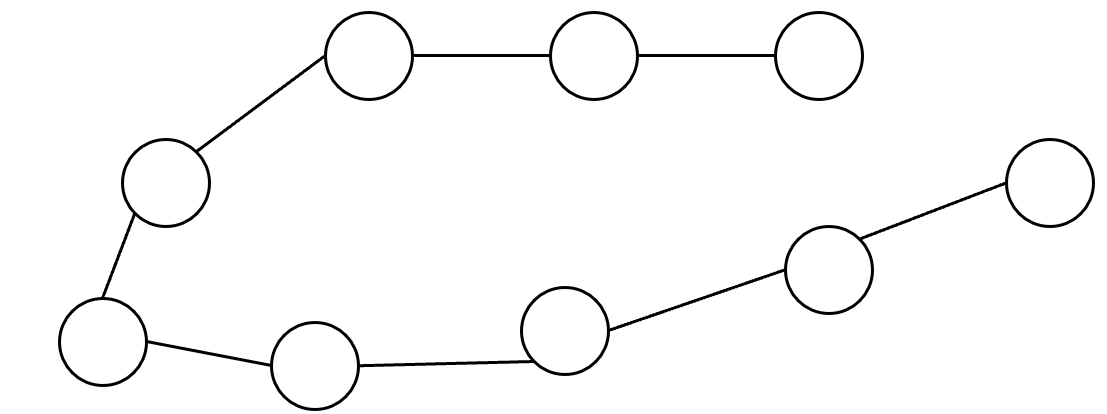
\includegraphics[width=0.52\textwidth]{assets/pics_and_ppts/ch5/习题04，N个顶点的连通图最少边数答案.png}
\end{center}
在此情况下，再少一条边，则图将不连通。显然此情况边数等于顶点数减一。即：\textbf{有N个顶点的无向图，要保证它是连通图，至少要有N-1条边。换句话说，
有N个顶点的无向图，若边数小于N-1，则它一定是不连通的。}

也可以这样理解：对于N个顶点、无边的无向图，显然有N个连通块。之后每添加1条边，一定能让两个本不连通的块连通起来。因此，添加N-1条边后，就只剩一个连通块了。\\

6. 选C：16。若N为15，则存在一种方式：将其中6个顶点通过这\(\frac{6\cdot (6-1)}{2} = 15\)条边连接为一个完全图，将第七个顶点孤立在外，使得图G不连通。而若N为16，
多出来的一条边一定可以让第七个顶点与另外6个连通。\\

7. 选A。图的邻接矩阵AdjM[i][j]存储的是编号为$i$的顶点到编号为$j$的顶点的边的信息。0表示无边，那么编号为$i$的顶点的度
就等于邻接矩阵第 \(i\) 行（或第 \(i\) 列）中非零元素的数量。\\

8. 选B。 如果是有向图，那么AdjM[i][*]，即第$i$行的非0元素数量，是顶点$i$的出度，而AdjM[*][i]，即第$i$列的非0元素数量，是顶点$i$的入度，二者加起来才是顶点$i$的度。\\

